%%
% 引言或背景
% 引言是论文正文的开端,应包括毕业论文选题的背景、目的和意义;对国内外研究现状和相关领域中已有的研究成果的简要评述;介绍本项研究工作研究设想、研究方法或实验设计、理论依据或实验基础;涉及范围和预期结果等。要求言简意赅,注意不要与摘要雷同或成为摘要的注解。
% modifier: 黄俊杰(huangjj27, 349373001dc@gmail.com)
% update date: 2017-04-15
%%

\chapter{绪论}
%定义,过去的研究和现在的研究,意义,与图像分割的不同,going deeper
\label{cha:introduction}
\section{选题背景与意义}
\label{sec:background}
% What is the problem
% why is it interesting and important
% Why is it hards, why do naive approaches fails
% why hasn't it been solved before
% what are the key components of my approach and results, also include any specific limitations,do not repeat the abstract
%contribution
随着医疗技术的进步,各种新型的医学影像设备已广泛应用在临床诊断中,其中包括计算机断层扫描(CT)、磁共振成像(MRI)、超声成像(UI)等。医学图像中含有非常有用的信息,医生可利用CT及其他医学图像来诊断患者病情,医学图像已逐渐成为临床诊断的主要依据,因此,对医学图像处理的研究具有重要意义。其中,医学图像分割是该领域的研究热点,属于语义分割的一种,图像分割将图像划分成多个解剖学意义的区域,并在此基础上可以计算相应区域的相关定量指标用于辅助临床诊断。

一般地,医学图像分割可以用集合论的术语描述\cite{liu2021review}:给定一张医学图像$I$以及相似性约束集合$C_i\ (i=1,2,\dots)$,对图像$I$的分割即得到其分划:
\begin{align}
    \bigcup_{\mathrm{x}=1}^{\mathrm{N}} R_{x}=\mathrm{I}, \quad R_{x} \cap R_{y}=\varnothing, \quad \forall x \neq y, x, y \in[1, N]
\end{align}
其中每个$R_x$中的所有像素都满足相似性约束$C_i\ (i=1,2,\dots)$,代表不同病理学意义的区域。利用传统的图像处理方法和机器学习方法来进行医学图像分割往往需要繁琐的特征工程或先验知识,而深度学习能够自动提取出复杂有效的特征,基于卷积神经网络的方法已经广泛应用在医学图像处理当中。

\begin{figure}
    \centering
    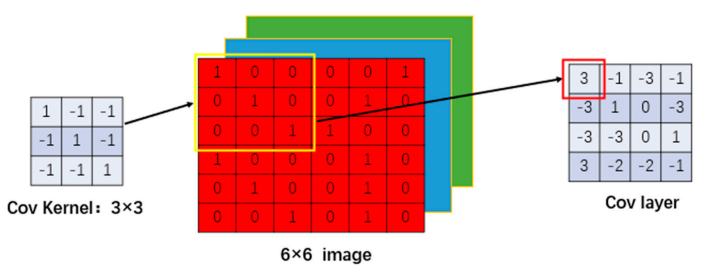
\includegraphics[width=\textwidth]{image/chap01/cnn.png}
    \caption{2D卷积神经网络卷积运算过程,图源\cite{liu2021review}}
    \label{fig:cnn}
\end{figure}
卷积神经网络已成功地应用于许多图像分类、目标检测和分割任务。假设输入图像的大小为$H\times W\times 3$,大小为$(h, w, c)$的卷积核在图像的空间维度进行滑动,在每个通道进行相应位置的卷积运算,具体的2D卷积神经网络计算过程如图\ref{fig:cnn}所示。由卷积神经网络,下采样层,激活函数组成的深层神经网络在医学图像分割中已取得了良好的效果\cite{ronneberger2015u,chen2014semantic,badrinarayanan2017segnet},其中U-Net\cite{ronneberger2015u}的使用最为广泛,对其结构的拓展仍为该领域的热门方向。

U-Net网络由一个U型网络和跳跃连接组成,如图\ref{fig:unet}。该U型网络类似一种编码器解码器的结构。编码器包含四个子模块,每个子模块包含两层卷积神经网络及用于下采样的最大池化层,对称地,解码器的四个子模块也包含两层神经网络及上采样层。同时,解码器每个子模块的输入由上个子模块的输出以及编码器中对称的子模块的输出跳跃连接组成,二者具有相同的分辨率,为的是结合网络结构低层和高层中的语义信息,帮助提取出图像中更复杂的结构,提升分割的准确率。
\begin{figure}
    \centering
    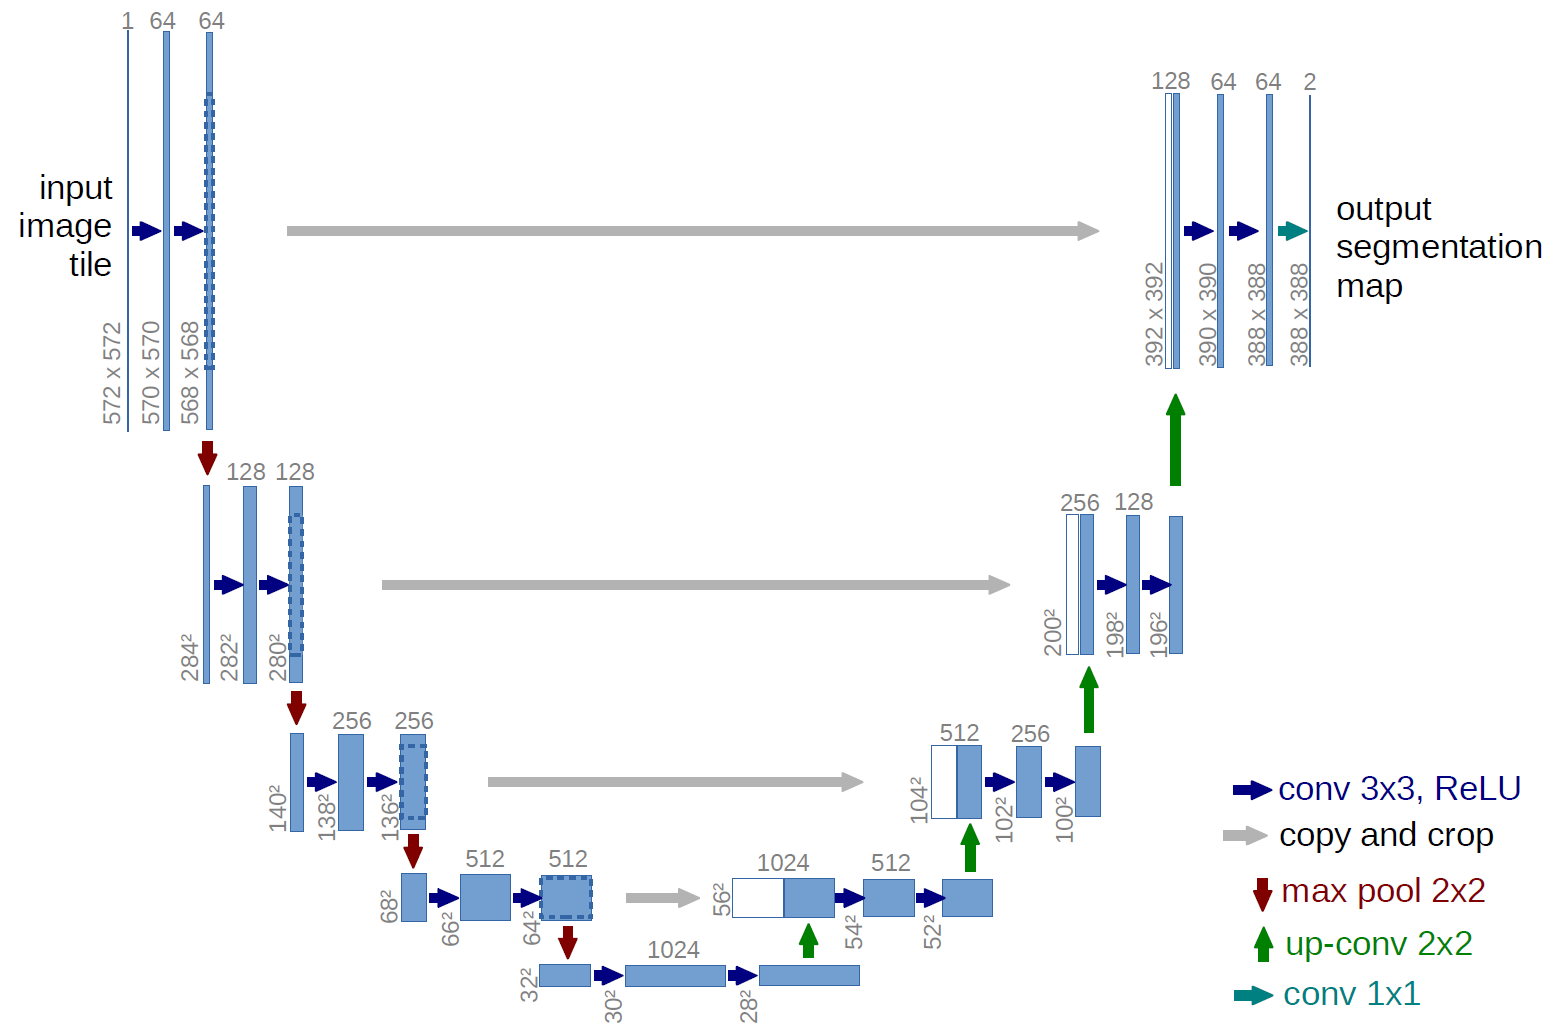
\includegraphics[width=0.8\textwidth]{image/chap01/u-net-architecture.png}
    \caption{U-Net网络结构,图源\cite{ronneberger2015u}}
    \label{fig:unet}
\end{figure}

在临床诊断中,多模态的医学图像常被用于辅助诊断,而医学图像的标注成本比较昂贵,专家标注一张完整的分割图像大约需要8小时\cite{zhuang2013challenges},解决这个问题的一种不失为有效的方法是基于学习的方法对一种模态的已有标注数据进行建模并用于另一种模态的图像分割。然而,机器学习方法通常假设训练集和测试集同属于一个数据分布,这个假设在该实际的临床场景中通常不成立,在训练集上训练好的模型在测试集上不能得到很好的泛化。先前的研究表明,测试误差会随着训练集和测试集的分布差异而增加\cite{ben2007analysis},这就是域位移问题,训练集(源域)和测试集(目标域)的分布具有一定的差异。在医学图像领域,由于各种成像模式具有不同的物理原理,异构域位移的情况更加常见和严重,如多中心,跨模态等,见图\ref{fig:hist}。在不需要目标域的带标注数据的情况下,无监督域自适应(Unsupervised Domain Adaptation,UDA)是解决由域位移带来的性能下降的一种方法。由于不需要额外的标注数据,UDA在医学图像领域中越来越受到关注。

在UDA的框架中,我们称带标注数据为源域,不带标注的数据为目标域,UDA的目的对齐源域和目标域数据的分布,一种方法是特征自适应\cite{long2017deep, sun2016deep, wu2020cf, wu2021unsupervised, dou2018pnp, tsai2018learning, vesal2021adapt},将不同模态的图像映射到一个模态不变的特征空间,另一种方法是图像自适应\cite{zhu2017unpaired},将图像从一种模态直接转换为有着相同解剖学结构的另一种模态。对于特征自适应,可以通过距离度量来显式地减小源域和目标域在特征空间上的分布差异,此外,也可以通过对抗学习来隐式地减小源域和目标域的差异。近期的研究\cite{hoffman2018cycada,chen2019synergistic}提出特征自适应和图像自适应从互补的角度来缓解域位移问题,二者有效地相结合能够改进域自适应的表现。此外,多模态的医学图像具有丰富的层次性特征,一些工作\cite{yang2019unsupervised, chartsias2019disentangled, pei2021disentangle}利用解耦表示学习来提取医学图像中的域不变特征以及域特定特征。
\begin{figure}
    \centering
    \begin{subfigure}{0.3\textwidth}
        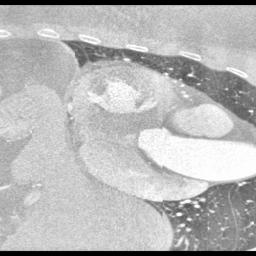
\includegraphics[width=.8\textwidth,height=.8\textwidth]{image/chap01/ct.jpeg}
        \caption{CT图}
        \label{hist:a}
    \end{subfigure}
    \hfill
    \begin{subfigure}{0.3\textwidth}
        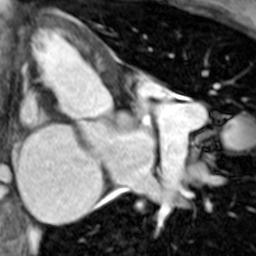
\includegraphics[width=.8\textwidth,height=.8\textwidth]{image/chap01/mr.jpeg}
        \caption{MRI图}
        \label{hist:b}
    \end{subfigure}
    \hfill
    \begin{subfigure}{0.3\textwidth}
        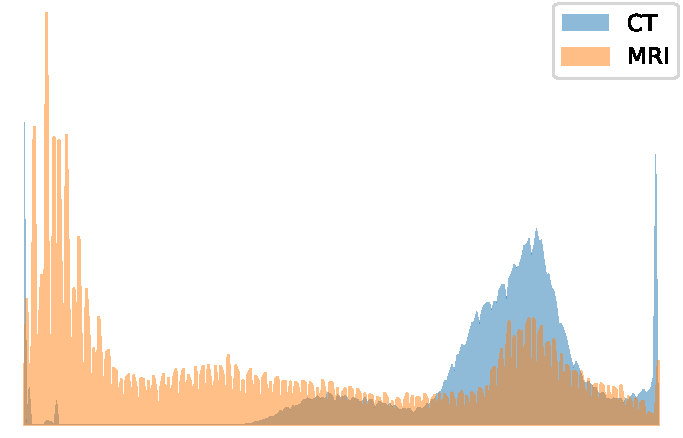
\includegraphics[width=\textwidth,height=.8\textwidth]{image/chap01/hist.pdf}
        \caption{灰度直方图}
        \label{hist:c}
    \end{subfigure}
    \caption{心脏的CT图,MRI图及其对应的灰度直方图}
    \label{fig:hist}
    \end{figure}


\section{本文方法概述}
\label{sec:contributions}
本文提出了一个新的UDA框架用于跨模态医学图像分割。该框架基于解耦表示学习来提取出不同模态的心脏图像的模态特征以及解剖学特征,结合图像自适应和特征自适应,进而利用不同模态的医学图像之间具有相似的解剖学特征来实现跨模态的医学图像分割。主要贡献如下:
\begin{itemize}
    \item 利用解耦表示学习提取出跨模态医学图像的模态特征和解剖学特征,进而实现非成对跨模态图像之间的转换。
    \item 在CT-MRI多模态心脏数据集进行相关实验,验证了方法的有效性。
\end{itemize}

\newpage
\section{本文的论文结构与章节安排}
\label{sec:arrangement}

本文共分为六章,各章节内容安排如下:

第一章绪论。简单说明了本文章的选题背景与意义。

第二章为本领域的相关工作。

第三章为本文方法的详细介绍。

第四章为实验与结果。

第五章为总结与展望。

